\section{Inteligência artificial}

\begin{frame}{Aprendizado de máquina}
	\begin{description}[aprendizado não-supervisionado]
		\item[Aprendizado supervisionado] utiliza pares de entrada-saída (rotulados) para aprender;
		\item[aprendizado não-supervisionado] tenta aprender padrões nos dados, como grupos de exemplos similares;
		\item[classificação] identifica a classe da informação;
		\note{exemplo classificação: identificar se um animal é cão ou gato\\}
		\item[agrupamento] determina classes agrupando informações similares em grupos (\textit{clusters})
		\note{exemplo agrupamento: agrupamento de filmes em gêneros\\}
		\item[regressão] prevê algum valor ou quantidade
		\note{exemplo regressão: prever o preço de ações ao longo do tempo\\}
		\item[redução de dimensionalidade] representa dados de várias dimensões em outras menores
		\note{exemplo redução de dimensionalidade: várias informações de um paciente sendo reduzidas às mais importantes para o diagnóstico de uma doença}
	\end{description}
\end{frame}

\subsection{Redes neurais}
\begin{frame}{Redes neurais}
	\begin{figure}
		\centering
		\caption{Arquiteturas do Perceptron}
		\label{fig:perceptrons}
		\begin{subfigure}[b]{0.3\textwidth}
			\caption{Perceptron}
			\label{fig:perceptron}
			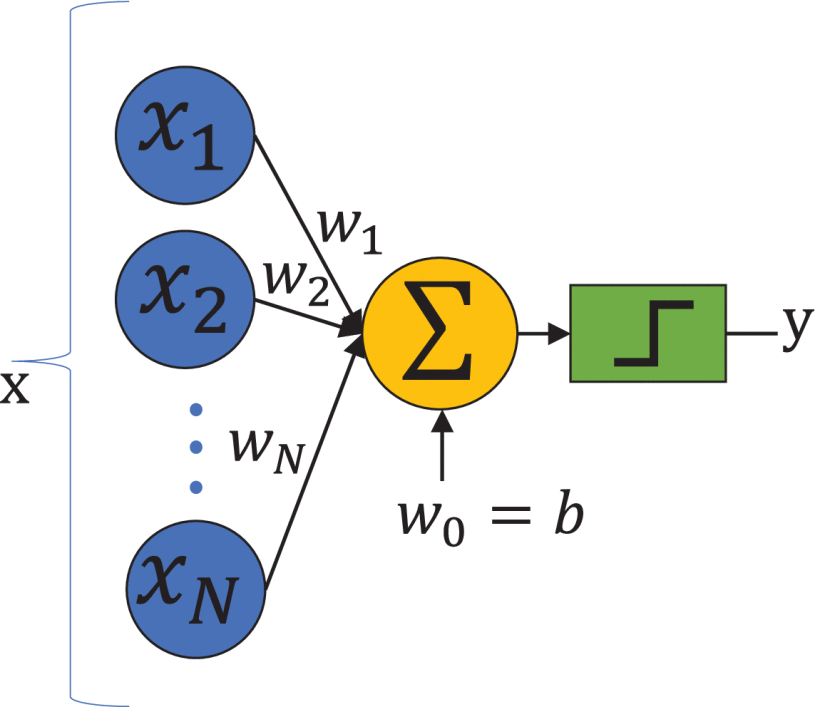
\includegraphics[width=\textwidth]{figs/perceptron}
		\end{subfigure}
		\qquad\qquad
		\begin{subfigure}[b]{0.3\textwidth}
			\caption{Perceptron de multi-camadas}
			\label{fig:mlp}
			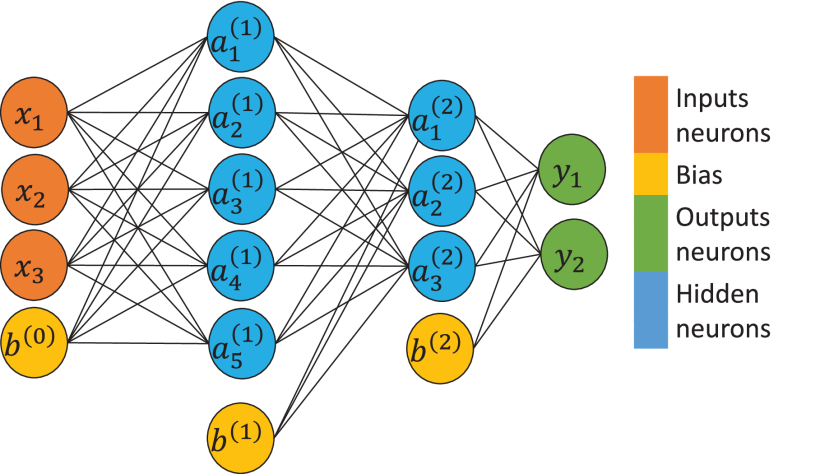
\includegraphics[width=\textwidth]{figs/mlp}
		\end{subfigure}
%		\fonte{\cite{parhi_brain-inspired_2020}}
	\end{figure}
	\note{perceptron: base do aprendizado de máquina\\}
	\note{$x_k$ é a resposta da sinapse $k$, $w_k$ é o peso da sinapse, $b$ é o \textit{bias} (viés, em português), um peso de referência que representa um conhecimento a priori, $\sigma$ é uma função de ativação não-linear, e $y$ é a saída do neurônio\\}
	\note{perceptron sozinho não é capaz de realizar tarefas de separação linear: MLP\\}
	\note{atualização dos pesos através do gradiente descendente (minimização do erro entre saída da rede e real)\\}
	\note{atualização com a metodologia da retropropagação: atualização das camadas finais em direção às iniciais\\}
	\note{quando a quantidade de camadas na rede é grande é chamada de rede neural profunda}
\end{frame}

\begin{frame}{Arquiteturas de redes neurais artificiais}
	\begin{itemize}
		\item \textit{Convolutional Neural Networks} (CNN, Redes neurais convolucionais)
		\note{CNN: possui camadas que implementam a operação matemática de convolução, aplicando um filtro no sinal, e camadas de sub-amostragem (\textit{downsampling}), chamadas de \textit{pooling}\\}
		\item \textit{Recurrent Neural Networks} (RNN, Redes neurais recorrentes)
		\note{RNN: possem a característica de processar os dados elemento a elemento, considerando também informações dos elementos passados, armazenados em pesos de conexões recorrentes, que funcionam como uma memória dinâmica para a rede\\}
		\item \textit{Hopfield Networks} (Redes Hopfield)
		\note{Hopfield: são redes treinadas para aprender padrões (memórias) dos dados de maneira associativa, baseado no princípio de Hebb \\}
		\item \textit{Autoencoder} (auto codificador)
		\note{autoencoder: redes que aprendem a representar os dados reduzindo sua dimensionalidade, diminuindo as camadas ocultas, e, posteriormente, recriando os dados originais\\}
		\item \textit{Long Short-Term Memory} (LSTM, memória longa de curto prazo)
		\note{LSTM: uma variação da RNN composta de 4~(quatro) blocos de memória, sendo um principal e os outros três, chamados de portões de entrada, esquecimento e saída, responsáveis por alterar o estado da célula como um todo}
	\end{itemize}
\end{frame}

\subsection{Redes neuromórficas}
\begin{frame}{Redes neuromórficas}
	\begin{columns}[t]
		\column{5cm}
			\begin{figure}[tb]
				\centering
				\caption{Arquitetura de redes neurais de disparo (SNN)}
				\label{fig:snn}
				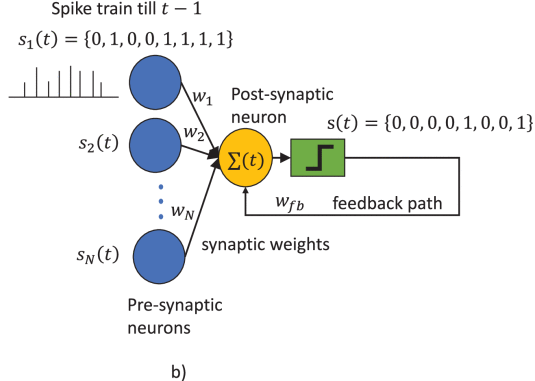
\includegraphics[width=\linewidth]{figs/snn}
%				\fonte{\cite{parhi_brain-inspired_2020}}
			\end{figure}
		\column{5cm}
			\begin{itemize}
				\item Distribui o processamento e memória em conjunto nos elementos de neurônio e sinapse;
				\note{von neumann: memória e processamento ficam separadas\\}
				\item informação codificada em sequências de potenciais de ação;
				\note{von neumann: codificação para sinais binários (0 e 1)\\}
				\item programas definidos pela estrutura da rede neural e seus parâmetros.
				\note{von neumann: programas escritos em instruções explícitas}
			\end{itemize}
	\end{columns}
\end{frame}

\begin{frame}{Redes neuromórficas}
	\begin{itemize}
		\item Usam, principalmente, neurônios do tipo integra-e-dispara;
		\item redes neurais convencionais podem ser convertidas em redes de disparo fazendo ajustes de pesos e normalizações;
		\item dados de entrada precisam ser codificados em disparos de potencial de ação;
		\note{codificações baseadas em taxa de disparo, ordem dos disparos ou temporalmente\\}
		\item o aprendizado frequentemente usa a STDP para o não-supervisionado, e uma versão do \textit{backpropagation} para o supervisionado, relacionando ativações das unidades de redes neurais com taxas de disparo.
		\note{há discussões sobre o treinamento com backprop na simulação do cérebro}\\
		\note{57 min}
	\end{itemize}
\end{frame}
